\documentclass{beamer}
\usepackage[utf8]{inputenc}
\usepackage[spanish]{babel}
\usepackage{listings}
\usepackage{multicol}
\usepackage{graphicx}
\lstloadlanguages{Ruby}
\lstset{%
  basicstyle=\ttfamily\small\color{black},
  commentstyle = \ttfamily\color{red},
  keywordstyle=\ttfamily\color{blue},
stringstyle=\color{orange}}

\begin{document}
\title{La primera abstracción funcional: lifting}
\author{Juan Pablo Santos}
\date{17 de octubre de 2015}

\begin{frame}
  \titlepage
\end{frame}

\begin{frame}
  \frametitle{Agenda}
  \tableofcontents
\end{frame}

\section{Funciones puras}
\begin{frame}
  \frametitle{Funciones puras}
  \begin{itemize}
    \item Mismos argumentos, mismo resultado.
    \item Evaluación sin efectos secundarios implicitos.
    \item No mantiene estado implicito entre invocaciones.
    \item No es muy útil.
  \end{itemize}
\end{frame}

\section{El método Array\#map}
\begin{frame}
  \frametitle{El método Array\#map}
  \begin{itemize}
    \item ¿Qué hace?
    \item Nueva colección
    \item Efectos secundarios
    \item Transformación de colecciones
    \item Bloques
    \item vs \#each
  \end{itemize}

\end{frame}

\section{El método \#map}
\begin{frame}[fragile]
  \frametitle{El método \#map}
  \begin{itemize}
    \item Expectativas
    \begin{itemize}
        \item Identidad
        \item Composición
    \end{itemize}
  \end{itemize}

  \begin{lstlisting}[language=Ruby, caption=Identidad de \#map]
    [1,2,3].map { |n| n } == [1,2,3]
  \end{lstlisting}

  \begin{lstlisting}[language=Ruby, caption=Composición de \#map]
    [1,2,3].map { |n| n*n }.map { |m| m + 1 }
    ==
    [1,2,3].map { |n| (n*n) + 1 }
  \end{lstlisting}

\end{frame}

\section{Adaptadores}
\begin{frame}[fragile]
  \frametitle{Adaptadores}
  \begin{itemize}
    \item Funciones sobre listas de valores.
    \item Funciones sobre valores.
    \item \#map como un adaptador. Funciones sobre valores a funciones
      sobre listas.
    \item ¿Listas vacias?
  \end{itemize}
\end{frame}

\section{¿Otros adaptadores?}
\begin{frame}[fragile]
  \frametitle{¿Otros adaptadores?}
  \begin{itemize}
    \item \begin{verbatim}Enumerable#map\end{verbatim} once again!
    \item Funciones sobre valores que pueden ser nil.
    \item Funciones sobre listas vacias.
    \item Funciones sobre valores.
    \item Funciones sobre listas con un solo valor.
  \end{itemize}
\end{frame}

\section{The billion dollar mistake}
\begin{frame}
  \frametitle{The billion dollar mistake}
  \begin{multicols}{2}
    \begin{quote}
      I call it my billion-dollar mistake. It was the invention of the
      null reference in 1965. [\ldots] But I couldn't resist the
      temptation to put in a null reference, simply because it was so
      easy to implement. This has led to innumerable errors,
      vulnerabilities, and system crashes, which have probably caused
      a billion dollars of pain and damage in the last forty years
    \end{quote}

    \columnbreak

    \begin{figure}
      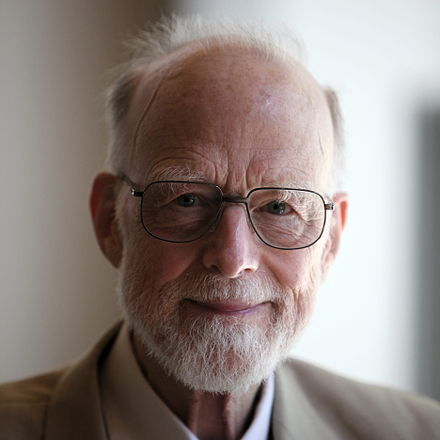
\includegraphics[scale=0.2]{hoare.jpg}
      \caption{Tony Hoare}
    \end{figure}
  \end{multicols}
\end{frame}

\section{Valores opcionales}
\begin{frame}[fragile]
  \frametitle{Valores opcionales}

  \begin{lstlisting}[language=Ruby]
    square = lambda { |n| n*n }
  \end{lstlisting}
  \begin{lstlisting}[language=Ruby]
    square(nil)
  \end{lstlisting}

  \begin{verbatim}
  undefined method `*' for nil:NilClass
  \end{verbatim}

  Funciones sobre listas vacias.
  \begin{lstlisting}[language=Ruby]
    [].map &square == []
  \end{lstlisting}
  Funciones sobre listas con un solo valor.
  \begin{lstlisting}
    [5].map &square == [25]
  \end{lstlisting}
  ¿Possibly? \ldots
\end{frame}

\section{ActiveRecord::QueryMethods\#where}
\begin{frame}[fragile]
  \frametitle{ActiveRecord::QueryMethods\#where}
  \lstinputlisting[language=Ruby]{repl_load.pry}
\end{frame}

\section{Possibly!}
\begin{frame}[fragile]
  \frametitle{Possibly!}
  \lstinputlisting[language=Ruby, firstline=1, lastline=18]{possibly_enumerable.rb}
\end{frame}

\begin{frame}[fragile]
  \frametitle{Possibly: Some}
  \lstinputlisting[language=Ruby, firstline=20, lastline=32]{possibly_enumerable.rb}
\end{frame}

\begin{frame}[fragile]
  \frametitle{Possibly: None}
  \lstinputlisting[language=Ruby, firstline=34, lastline=42]{possibly_enumerable.rb}
\end{frame}

\section{Cadenas}
\begin{frame}[fragile]
  \frametitle{Cadenas}
  \lstinputlisting[language=Ruby, firstline=1, lastline=10]{chains.rb}
\end{frame}

\begin{frame}[fragile]
  \frametitle{Cadenas}
  \lstinputlisting[language=Ruby, firstline=1, lastline=10]{chains_ary.rb}
\end{frame}

\begin{frame}[fragile]
  \frametitle{Cadenas}
  \lstinputlisting[language=Ruby, firstline=12, lastline=26]{concurrent_chain.rb}
\end{frame}

\end{document}
